\section{Squark and Gluino Production at Tree Level}
Comment on sgluon production: which channels, calculate cross section for at least one configuration of masses.\\
In this chapter the production of strongly interacting supersymmetric particles\footnote{The production of sgluons is excluded from the analysis for their mass is chosen to be too large to significantly produce them.} in the MRSSM is considered. The various processes and their associated cross section is compared to their analogues in the MSSM.


\subsection{Partonic Processes} 
\begin{figure}[!htbp]
\begin{center}
\begin{tikzpicture}[line width=1.0 pt, scale=1.3, arrow/.style={thick,->,shorten >=2pt,shorten <=2pt,>=stealth}]
	\draw[fermion] (-1,0.5)--(-0.42,0);
	\draw[fermionbar] (-1,-0.5)--(-0.42,0);
	\draw[gluon] (-0.42,0)--(0.42,0); 
	\draw[scalar] (0.42,0)--(1,0.5);
	\draw[scalarbar] (0.42,0)--(1,-0.5);
	\draw[arrow] (-1,0.7)--(-0.5,0.26);
	\node at (-0.75,0.8) {$k_a$};
	\draw[arrow] (-1,-0.7)--(-0.5,-0.26);
	\node at (-0.75,-0.8) {$k_b$};
	\draw[arrow] (0.5,0.26)--(1,0.7);
	\node at (0.75,0.8) {$p_1$};
	\draw[arrow] (0.5,-0.26)--(1,-0.7);
	\node at (0.75,-0.8) {$p_2$};
\begin{scope}[shift={(3,0)}]
	\draw[fermion] (-1,0.5)--(0,0.5);
	\draw[fermionbar] (-1,-0.5)--(0,-0.5);
	\draw[fermionnoarrow] (0,0.5)--(0,-0.5);
	\draw[gluon] (0,0.5)--(0,-0.5); 
	\draw[scalar] (0,0.5)--(1,0.5);
	\draw[scalarbar] (0,-0.5)--(1,-0.5);
\end{scope}
\end{tikzpicture}
%\caption{Tree level diagrams for $q\overline{q} \to \tilde{q}\tilde{q}^\dagger$}
\end{center}
%\end{figure}
%\begin{figure}[!htbp]
\begin{center}
\begin{tikzpicture}[line width=1.0 pt, scale=1.3]
    \node at (0,0) {};
\begin{scope}[shift={(0,-1)}]
	\draw[gluon] (-1,0.5)--(-0.42,0);
	\draw[gluon] (-1,-0.5)--(-0.42,0);
	\draw[gluon] (-0.42,0)--(0.42,0); 
	\draw[scalar] (0.42,0)--(1,0.5);
	\draw[scalarbar] (0.42,0)--(1,-0.5);
\begin{scope}[shift={(3,0)}]
	\draw[gluon] (-1,0.5)--(0,0.5);
	\draw[gluon] (-1,-0.5)--(0,-0.5);
	\draw[scalarbar] (0,0.5)--(0,-0.5);
	\draw[scalar] (0,0.5)--(1,0.5);
	\draw[scalarbar] (0,-0.5)--(1,-0.5);
\end{scope}
\begin{scope}[shift={(6,0)}]
	\draw[gluon] (-1,0.5)--(0,0.5);
	\draw[gluon] (-1,-0.5)--(0,-0.5);
	\draw[scalar] (0,0.5)--(0,-0.5);
	\draw[scalarnoarrow] (0,0.5)--(0.4,0.1);
	\draw[scalarbar] (0.6,-0.1)--(1,-0.5);
	\draw[scalarnoarrow] (0,-0.5)--(0.5,0);
	\draw[scalar] (0.5,0)--(1,0.5);
\end{scope}
\begin{scope}[shift={(9,0)}]
	\draw[gluon] (-1,0.5)--(0,0);
	\draw[gluon] (-1,-0.5)--(0,0);
	\draw[scalarbar] (0,0)--(1,-0.5);
	\draw[scalar] (0,0)--(1,0.5);
\end{scope}
\end{scope}
\end{tikzpicture}
%\caption{Tree level diagrams for $GG \to \tilde{q}\tilde{q}^\dagger$}
\end{center}
%\end{figure}
%\begin{figure}[!htbp]
\begin{center}
\begin{tikzpicture}[line width=1.0 pt, scale=1.3]
    \node at (0,0) {};
\begin{scope}[shift={(0,-1)}]
	\draw[fermion] (-1,0.5)--(0,0.5);
	\draw[fermion] (-1,-0.5)--(0,-0.5);
	\draw[gluon] (0,0.5)--(0,-0.5);
	\draw[fermionnoarrow] (0,0.5)--(0,-0.5);
	\draw[scalar] (0,0.5)--(1,0.5);
	\draw[scalar] (0,-0.5)--(1,-0.5);;
\begin{scope}[shift={(3,0)}]
	\draw[fermion] (-1,0.5)--(0,0.5);
	\draw[fermion] (-1,-0.5)--(0,-0.5);
	\draw[gluon] (0,0.5)--(0,-0.5);
	\draw[fermionnoarrow] (0,0.5)--(0,-0.5);
	\draw[scalarnoarrow] (0,0.5)--(0.4,0.1);
	\draw[scalar] (0.6,-0.1)--(1,-0.5);
	\draw[scalarnoarrow] (0,-0.5)--(0.5,0);
	\draw[scalar] (0.5,0)--(1,0.5);
\end{scope}
\end{scope}
\end{tikzpicture}
%\caption{Tree level diagrams for $qq \to \tilde{q}\tilde{q}$}
\end{center}
%\end{figure}
%\begin{figure}[!htbp]
\begin{center}
\begin{tikzpicture}[line width=1.0 pt, scale=1.3]
    \node at (0,0) {};
\begin{scope}[shift={(0,-1)}]
	\draw[fermion] (-1,0.5)--(-0.42,0);
	\draw[fermionbar] (-1,-0.5)--(-0.42,0);
	\draw[gluon] (-0.42,0)--(0.42,0); 
	\draw[gluon] (0.42,0)--(1,0.5);
	\draw[fermionnoarrow] (0.42,0)--(1,0.5);
	\draw[gluon] (0.42,0)--(1,-0.5);
	\draw[fermionnoarrow] (0.42,0)--(1,-0.5);
\begin{scope}[shift={(3,0)}]
	\draw[fermion] (-1,0.5)--(0,0.5);
	\draw[fermionbar] (-1,-0.5)--(0,-0.5);
	\draw[scalar] (0,0.5)--(0,-0.5);
	\draw[gluon] (0,0.5)--(1,0.5);
	\draw[fermionnoarrow] (0,0.5)--(1,0.5);
	\draw[gluon] (0,-0.5)--(1,-0.5);
	\draw[fermionnoarrow] (0,-0.5)--(1,-0.5);
\end{scope}
\begin{scope}[shift={(6,0)}]
	\draw[fermion] (-1,0.5)--(0,0.5);
	\draw[fermionbar] (-1,-0.5)--(0,-0.5);
	\draw[scalar] (0,0.5)--(0,-0.5);
	\draw[gluon] (0,0.5)--(0.4,0.1);
	\draw[fermionnoarrow] (0,0.5)--(0.4,0.1);
	\draw[gluon] (0.6,-0.1)--(1,-0.5);
	\draw[fermionnoarrow] (0.6,-0.1)--(1,-0.5);
	\draw[gluon] (0,-0.5)--(1,0.5);
	\draw[fermionnoarrow] (0,-0.5)--(1,0.5);
\end{scope}
\end{scope}
\end{tikzpicture}
%\caption{Tree level diagrams for $q\overline{q} \to \tilde{g}\overline{\tilde{g}}$}
\end{center}
%\end{figure}
%\begin{figure}[!htbp]
\begin{center}
\begin{tikzpicture}[line width=1.0 pt, scale=1.3]
    \node at (0,0) {};
\begin{scope}[shift={(0,-1)}]
	\draw[gluon] (-1,0.5)--(-0.42,0);
	\draw[gluon] (-1,-0.5)--(-0.42,0);
	\draw[gluon] (-0.42,0)--(0.42,0); 
	\draw[gluon] (0.42,0)--(1,0.5);
	\draw[fermionnoarrow] (0.42,0)--(1,0.5);
	\draw[gluon] (0.42,0)--(1,-0.5);
	\draw[fermionnoarrow] (0.42,0)--(1,-0.5);
\begin{scope}[shift={(3,0)}]
	\draw[gluon] (-1,0.5)--(0,0.5);
	\draw[gluon] (-1,-0.5)--(0,-0.5);
	\draw[gluon] (0,0.5)--(0,-0.5);	
	\draw[fermionnoarrow] (0,0.5)--(0,-0.5);
	\draw[gluon] (0,0.5)--(1,0.5);
	\draw[fermionnoarrow] (0,0.5)--(1,0.5);
	\draw[gluon] (0,-0.5)--(1,-0.5);
	\draw[fermionnoarrow] (0,-0.5)--(1,-0.5);
\end{scope}
\begin{scope}[shift={(6,0)}]
	\draw[gluon] (-1,0.5)--(0,0.5);
	\draw[gluon] (-1,-0.5)--(0,-0.5);
	\draw[gluon] (0,0.5)--(0,-0.5);
	\draw[fermionnoarrow] (0,0.5)--(0,-0.5);
	\draw[gluon] (0,0.5)--(0.4,0.1);
	\draw[fermionnoarrow] (0,0.5)--(0.4,0.1);
	\draw[gluon] (0.6,-0.1)--(1,-0.5);
	\draw[fermionnoarrow] (0.6,-0.1)--(1,-0.5);
	\draw[gluon] (0,-0.5)--(1,0.5);
	\draw[fermionnoarrow] (0,-0.5)--(1,0.5);
\end{scope}
\end{scope}
\end{tikzpicture}
%\caption{Tree level diagrams for $GG \to \tilde{g}\overline{\tilde{g}}$}
\end{center}
%\end{figure}
%\begin{figure}[!htbp]
\begin{center}
\begin{tikzpicture}[line width=1.0 pt, scale=1.3]
    \node at (0,0) {};
\begin{scope}[shift={(0,-1)}]
	\draw[fermion] (-1,0.5)--(-0.42,0);
	\draw[gluon] (-1,-0.5)--(-0.42,0);
	\draw[fermion] (-0.42,0)--(0.42,0); 
	\draw[scalar] (0.42,0)--(1,0.5);
	\draw[gluon] (0.42,0)--(1,-0.5);
	\draw[fermionnoarrow] (0.42,0)--(1,-0.5);
\begin{scope}[shift={(3,0)}]
	\draw[fermion] (-1,0.5)--(0,0.5);
	\draw[gluon] (-1,-0.5)--(0,-0.5);
	\draw[gluon] (0,0.5)--(0,-0.5);	
	\draw[fermionnoarrow] (0,0.5)--(0,-0.5);
	\draw[scalar] (0,0.5)--(1,0.5);
	\draw[gluon] (0,-0.5)--(1,-0.5);
	\draw[fermionnoarrow] (0,-0.5)--(1,-0.5);
\end{scope}
\begin{scope}[shift={(6,0)}]
	\draw[fermion] (-1,0.5)--(0,0.5);
	\draw[gluon] (-1,-0.5)--(0,-0.5);
	\draw[scalar] (0,0.5)--(0,-0.5);
	\draw[gluon] (0,0.5)--(0.4,0.1);
	\draw[fermionnoarrow] (0,0.5)--(0.4,0.1);
	\draw[gluon] (0.6,-0.1)--(1,-0.5);
	\draw[fermionnoarrow] (0.6,-0.1)--(1,-0.5);
	\draw[gluon] (0.6,-0.1)--(1,-0.5);
	\draw[fermionnoarrow] (0.6,-0.1)--(1,-0.5);
	\draw[scalarnoarrow] (0,-0.5)--(0.5,0);
	\draw[scalar] (0.5,0)--(1,0.5);
\end{scope}
\end{scope}
\end{tikzpicture}
\caption{Tree level diagrams for squark and gluino production at tree level in the MRSSM. The processes $GG \to \tilde{q}\overline{\tilde{q}}$ and $qG \to \tilde{q}\tilde{g}$ are identical to those in the MSSM. The processes $q\overline{q} \to \tilde{q}\overline{\tilde{q}}$ and $qq \to \tilde{q}\tilde{q}$ involve the production of less chiralities than in the MSSM. Also in the $q\tilde{q} \to \tilde{g}\overline{\tilde{g}}$ channel only half of the t-channel squark chiralities occur in the MRSSM. (Anti-)Gluino production via initial gluons $GG \to \tilde{g}\overline{\tilde{g}}$ proceeds via the same diagrams like in the MSSM but its cross section is twice as much in the MRSSM for gluino and antigluino are distinguishable particles.}\label{fig:TreeDiagrams}
\end{center}
\end{figure}
For the calculation the top quark is excluded from the initial state as it is too heavy to be significantly present in hadrons. %Therefore its pdf is approximately zero. 
For consistency reasons also the stop is excluded from the final states. One therefore deals with $n_f-1 = 5$ quark flavors. Using the Feynman rules in the Appendix one obtains the following sums over absolute squared Feynman amplitudes.
\begin{align}
\sum|\mathcal{M}^B|^2(q_i\overline{q}_j \to \tilde{q}\tilde{q}^\dagger) &= \delta_{ij}  \left[ 8 N_c C(F) g_s^4\frac{(n_f-1)}{s^2} + 4 N_c C(F) \hat{g}_s^4\frac{1}{t_{\tilde{g}}^2} - 8 C(F)g_s^2\hat{g}_s^2\frac{1}{ t_{\tilde{g}} s} \right] (tu-m_{\tilde{q}}^4)\nonumber\\
 &+ (1-\delta_{ij}) 4 N_c C(F) \hat{g}_s^4\frac{tu-m_{\tilde{q}}^4}{t_{\tilde{g}}^2} \\
\sum|\mathcal{M}^B|^2(GG \to \tilde{q}\tilde{q}^\dagger) &= 4 (n_f-1) g_s^4 \left[ 2N_c^2C(F) \left(1 - 2\frac{t_{\tilde{q}}u_{\tilde{q}}}{s^2} \right)- 2C(F) \right]\nonumber\\
& \left[ 1 - \epsilon - 2\frac{s m_{\tilde{q}}^2}{t_{\tilde{q}}u_{\tilde{q}}} \left( 1-\frac{s m_{\tilde{q}}^2}{t_{\tilde{q}}u_{\tilde{q}}} \right)\right]\\
\sum|\mathcal{M}^B|^2(q_i q_j \to \tilde{q}\tilde{q}) &= \delta_{ij} 2\hat{g}_s^4 N_c C(F)\left[ \frac{1}{t_{\tilde{g}}^2} + \frac{1}{u_{\tilde{g}}^2} \right] (tu-m_{\tilde{q}}^4)\nonumber\\ 
& + (1-\delta_{ij}) 4 \hat{g}_s^4 N_c C(F) \frac{tu-m_{\tilde{q}}^4}{t_{\tilde{g}}^2}\\
\sum|\mathcal{M}^B|^2(q\overline{q} \to \tilde{g}\overline{\tilde{g}}) &=  8 N_c^2 C(F) g_s^4 \left[ \frac{2m_{\tilde{g}}^2 s + t_{\tilde{g}}^2 + u_{\tilde{g}}^2}{s^2} -\epsilon \right]\nonumber\\
& + 4 N_c^2 C(F) g_s^2 \hat{g}_s^2 \left[ \frac{m_{\tilde{g}}^2 s + t_{\tilde{g}}^2}{s t_{\tilde{q}}} + \frac{m_{\tilde{g}}^2 s + u_{\tilde{g}}^2}{su_{\tilde{q}}} + \epsilon\left( \frac{t_{\tilde{g}}}{t_{\tilde{q}}} + \frac{u_{\tilde{g}}}{u_{\tilde{q}}} \right) \right]\nonumber\\
& + 2C(F)(N_c^2-1) \hat{g}^4_s \left( \frac{t_{\tilde{g}}^2}{t_{\tilde{q}}^2} + \frac{u_{\tilde{g}}^2}{u_{\tilde{q}}^2} \right)\\
%& + 2 \hat{g}_s^4\left[ 2 N_c^2 C(F) \left( \frac{t_{\tilde{g}}^2}{t_{\tilde{q}}^2} + \frac{u_{\tilde{g}}^2}{u_{\tilde{q}}^2} \right) + 2 C(F) \left( 2\frac{m_{\tilde{g}}^2 s}{t_{\tilde{q}}u_{\tilde{q}}} - \frac{t_{\tilde{g}}^2}{t_{\tilde{q}}^2} - \frac{u_{\tilde{g}}^2}{u_{\tilde{q}}^2} \right) \right]\\
\sum|\mathcal{M}^B|^2(GG \to \tilde{g}\overline{\tilde{g}}) &=  16 N_c^3 C(F) g_s^4 \left( 1- \frac{t_{\tilde{g}}u_{\tilde{g}}}{s^2} \right)\nonumber\\
&\left[ \frac{s^2}{t_{\tilde{g}}u_{\tilde{g}}}(1-\epsilon)^2-2(1-\epsilon) + 4\frac{m_{\tilde{g}}^2 s}{t_{\tilde{g}}u_{\tilde{g}}}\left(1-\frac{m_{\tilde{g}}^2 s}{t_{\tilde{g}}u_{\tilde{g}}}  \right) \right]\\
\sum|\mathcal{M}^B|^2(qg \to \tilde{q}\tilde{g}) &=  2g_s^2\hat{g}_s^2 \left[ 2 N_c^2 C(F) \left(1-2\frac{s u_{\tilde{q}}}{t_{\tilde{g}}^2}\right) - 2C(F) \right] \nonumber\\
&\left[ (-1+\epsilon)\frac{t_{\tilde{g}}}{s} + \frac{2(m_{\tilde{g}}^2-m_{\tilde{q}}^2)t_{\tilde{g}}}{s u_{\tilde{q}}}\left( 1+\frac{m_{\tilde{q}}^2}{u_{\tilde{q}}} + \frac{m_{\tilde{g}}^2}{t_{\tilde{g}}} \right) \right]
\end{align}
In view of the renormalization to be performed at the 1-loop level the results are given in $D = 4 - 2\epsilon$ dimensions and it has been distinguished between the gauge coupling $g_s$ from the gluon-quark-quark vertex and its supersymmetric analogue $\hat{g}_s$ from the gluino-squark-quark vertex. The usual Mandelstam variables $s,t,u$ and the following modifications of them are used\footnote{The kinematics of the process is like denoted in fig. \ref{fig:TreeDiagrams}.}
\begin{align}
& s = (k_a + k_b)^2 = (p_1 + p_2)^2\nonumber\\
& t = (k_a - p_1)^2 = (k_b - p_2)^2\nonumber\\
& u = (k_a - p_2)^2 = (k_a - p_2)^2\nonumber\\
& t_{\tilde{g}} = t - m_{\tilde{g}}^2 && t_{\tilde{q}} = t- m_{\tilde{q}}^2\nonumber\\
& u_{\tilde{g}} = u - m_{\tilde{g}}^2 && u_{\tilde{q}} = u- m_{\tilde{q}}^2
\end{align}



\subsection{Partonic Cross Sections}
Having calculated the absolute squared Feynman amplitudes one obtains the partonic cross sections (see Appendix \ref{sec:cross_section}) via
\begin{align}
\frac{\mbox{d}^2 \sigma^B}{\mbox{d}t\ \mbox{d}u} =& \frac{K_{ab}}{s^2} \frac{\pi S_{\epsilon}}{\Gamma(1-\epsilon)} \left[ \frac{tu-m_1^2m_2^2}{\mu^2 s}\right]^{-\epsilon} \Theta(tu-m_1^2m_2^2)\nonumber\\
&\ \Theta(s-4m^2) \delta(s+t+u-m_1^2-m_2^2) \sum |\mathcal{M}^B|^2\label{eq:sigma_tree}
\end{align}
The leading order cross sections are
\begin{align}
\sigma^B(q_i \overline{q}_j \to \tilde{q}\tilde{q}^\dagger) &= \delta_{ij}  \frac{g_s^4}{16\pi s} (n_f-1) \left[ \frac{4}{27} - \frac{16 m_{\tilde{q}}^2}{27s} \right]\nonumber\\
&+ \delta_{ij} \frac{g_s^2\hat{g}_s^2}{16\pi s}  \left[ \left( \frac{4}{27} + \frac{8 m_-^2}{27 s} \right)\beta_{\tilde{q}}  + \left( \frac{8m_{\tilde{g}}^2}{27s} + \frac{8m_-^4}{27s^2} \right)L_1 \right]\nonumber\\
& + \frac{\hat{g}_s^4}{16\pi s} \left[ -\frac{8}{9}\beta_{\tilde{q}} + \left( -\frac{4}{9} - \frac{8m_-^2}{9s} \right)L_1 \right]\\
\sigma^B(GG \to \tilde{q}\tilde{q}^\dagger) &= \frac{(n_f-1) g_s^4}{16\pi s} \left[ \left(\frac{5}{24} + \frac{31 m_{\tilde{q}}^2}{12s}\right)\beta_{\tilde{q}} + \left( \frac{4m_{\tilde{q}}^2}{3s} + \frac{m_{\tilde{q}}^4}{3s^2} \right) \ln \frac{1-\beta_{\tilde{q}}}{1+\beta_{\tilde{q}}} \right]\\
\sigma^B(q_i q_j \to \tilde{q}\tilde{q}) &= \frac{\hat{g}_s^4}{16\pi s} \left[ -\frac{8}{9}\beta_{\tilde{q}} +  \left( -\frac{4}{9} - \frac{8m_-^2}{9s} \right)L_1 \right]\\
\sigma^B(q \overline{q} \to \tilde{g}\overline{\tilde{g}}) &= \frac{g_s^4}{16\pi s} \left[ \frac{16}{9} + \frac{32m_{\tilde{g}}^2}{9s} \right] \beta_{\tilde{g}}\nonumber\\
& + \frac{\hat{g}_s^2 g_s^2}{16\pi s}  \left[ \left( -\frac{4}{3}-\frac{8m_-^2}{3s} \right)\beta_{\tilde{g}} + \left( \frac{8 m_{\tilde{g}}^2}{3s} + \frac{8m_-^4}{3s^2} \right) L_2 \right]\nonumber\\
& + \frac{\hat{g}_s^4}{16\pi s} \left[ \left( \frac{32}{27} + \frac{32 m_-^4}{27(m_-^4 + m_{\tilde{q}}^2s)} \right)\beta_{\tilde{g}} - \frac{64m_-^2}{27s}L_2 \right]\label{eq:qqbar_to_sgsgbar}\\
\sigma^B(GG \to \tilde{g}\overline{\tilde{g}}) &= \frac{g_s^4}{16\pi s} \left[ \left( -6 - \frac{51 m_{\tilde{g}}^2}{2s} \right)\beta_{\tilde{g}} + \left( -\frac{9}{2} - \frac{18 m_{\tilde{g}}^2}{s} + \frac{18 m_{\tilde{g}}^4}{s^2} \right)\ln \frac{1-\beta_{\tilde{g}}}{1+\beta_{\tilde{g}}} \right]\\
\sigma^B(q G \to \tilde{q} \tilde{g}) &= \frac{g_s^2\hat{g}_s^2}{16\pi s} \left[ \frac{\kappa}{s}\left( -\frac{7}{9} - \frac{32 m_{-}^2}{9s} \right) + \left( -\frac{8m_-^2}{9s} + \frac{2m_{\tilde{q}}^2m_-^2}{s^2} + \frac{8 m_-^4}{9s^2} \right)L_3\right.\nonumber\\
&+\left. \left( -1-\frac{2m_-^2}{s} + \frac{2m_{\tilde{q}}m_-^2}{s^2} \right)L_4 \right]
\end{align}
where the abbreviations \cite{Beenakker:1996ch} 
\begin{align}
&\beta_{\tilde{q}} = \sqrt{1-\frac{4 m_{\tilde{q}}^2}{s}} && \beta_{\tilde{g}} = \sqrt{1-\frac{4 m_{\tilde{g}}^2}{s}}\nonumber\\
&m_-^2 = m_{\tilde{g}}^2 - m_{\tilde{q}}^2 && \kappa = \sqrt{(s-m_{\tilde{g}}^2-m_{\tilde{q}}^2)^2-4m_{\tilde{g}}^2m_{\tilde{q}}^2}\nonumber\\
& L_1 = \ln \frac{s+2m_-^2 - s\beta_{\tilde{q}}}{s+2m_-^2 + s\beta_{\tilde{q}}} && L_2= \ln \frac{s - 2m_-^2 - s\beta_{\tilde{g}}}{s - 2m_-^2 + s\beta_{\tilde{g}}}\nonumber\\
& L_3 = \ln \frac{s - m_-^2 - \kappa}{s - m_-^2 + \kappa} && L_4= \ln \frac{s + m_-^2 - \kappa}{s + m_-^2 + \kappa}
\end{align}
are used. The comparison of the cross sections of the MRSSM with those of the MSSM is postponed until the next subsection where the confinement of quarks and gluons within hadrons is accounted for.



\subsection{Hadronic Cross Section}
factorization (pictorial explanation in factorization paper chapter 1.4 and Dissertori and Seymour, Marx page 24 below)\\
Quarks, anti-quarks and gluons are no free particles but are confined within hadrons. As hadrons consist of a variety of the just mentioned partons which share the hadron's momentum one does not have a definite initial state which is assumed in the previous subsection. Fortunately the hadronic cross section for the production of a final state $X$, e.g. $X = \tilde{q} \tilde{q}$, can be obtained by convolving the partonic cross section with the parton density functions of the initial partons.
\begin{align}
\sigma^B_{\mathrm{Had}}(P_1 P_2 \to X) = \int \mbox{d}x_1 \mbox{d}x_2\ f_{P_1/H_1}(x_1) f_{P_2/H_2}(x_2)\ \sigma^B_{\mathrm{Part}} (P_1 P_2 \to X, s = x_ 1x_2 S).
\end{align}
As the production of the final state $X$ may proceed via various initial partons one has to sum over all possible possibilities arising from the initial hadrons $H_1$ and $H_2$:
\begin{align}
\sigma^B_{\mathrm{Had}}(H_1 H_2 \to X) = \sum_{i,j} \sigma^B_{\mathrm{Had}}(P_1 P_2 \to X).
\end{align}
To get an intuitive idea of this factorization consider the hadrons as extended objects consisting of partons\footnote{The proton is considered as composed of three valence quarks: Two up-quarks and one down-quark. In addition there are gluons and seaquarks, i.e. virtual quark-antiquark pairs.} which are permanently interacting which each other. Now consider two colliding hadrons in their center-of-mass frame. Due to Lorentz contraction the hadrons appear as thin discs and the parton's mutual interactions are time-delayed within this frame. This effectively means that a hadron at the time of collision is virtually frozen.\\
maybe picture of colliding disks\\
This in turn implies that the hadron consists at the time of collision of a definite number of partons which can be thought of as carrying a definite fraction of the hadron's momentum $p_{\mathrm{Part}} = x p_{\mathrm{Had}}$ with $x \in \left(0, 1 \right)$. The parton density function $f_{P/H}(x)$ can therefore be understood as the probability of finding a parton $P$ within the hadron $H$ carrying $x$ of its momentum. See \cite{Brock:1993sz} for how to ascertain parton density functions\\
Fig. ... shows a parton density function set for the proton. One can see that the partons most probable to carry a high fraction of momentum are the valence quarks. For lower values of $x$ gluons constitute the major component of the proton.\\
\begin{figure}[!htpb]
\begin{center}
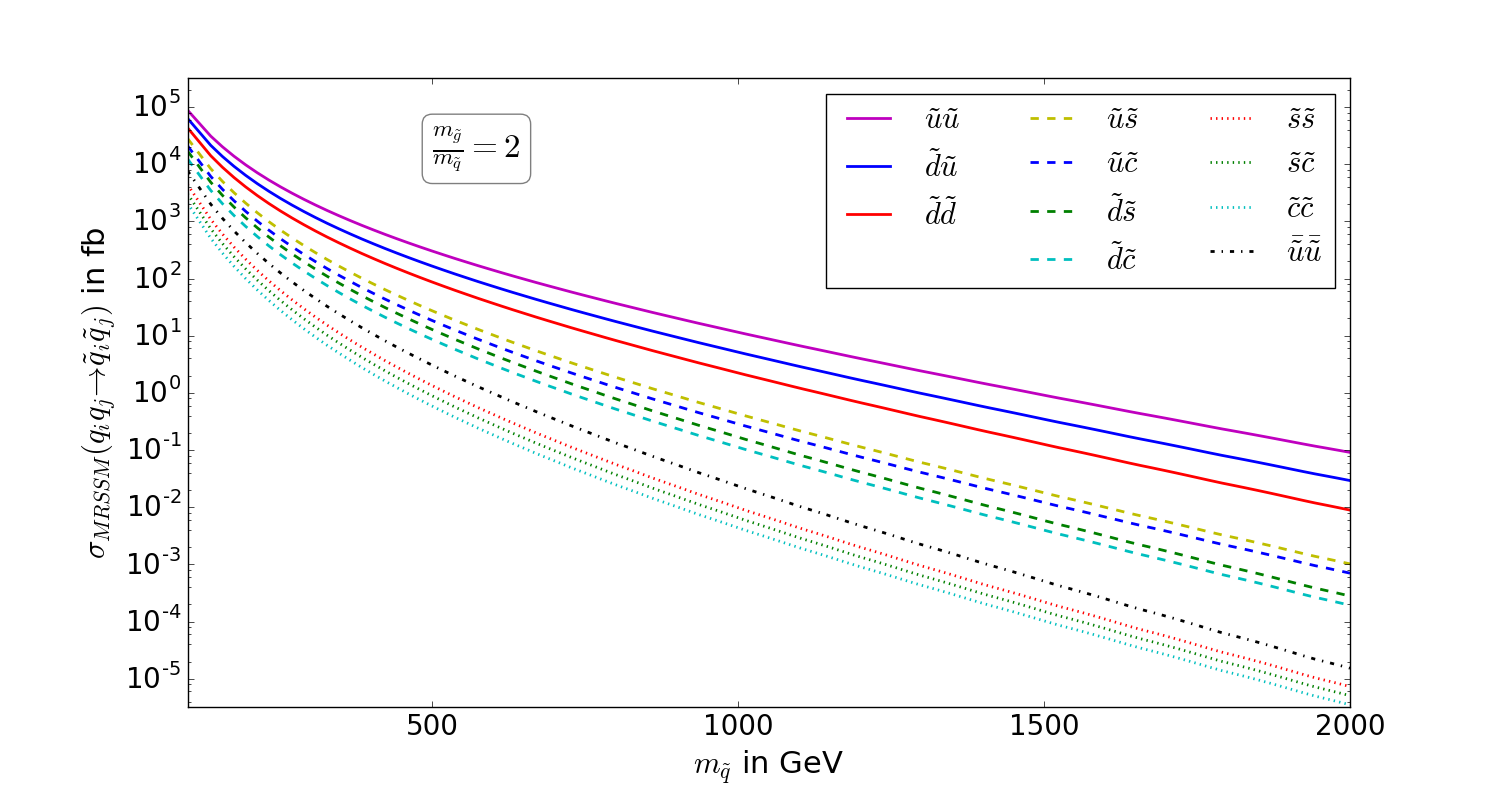
\includegraphics[scale=.45]{figures/MRSSM:q+q->sq+sq_mr=2_seperated}
\caption{Hadronic cross section for squark production in the MRSSM at the LHC at $\sqrt{S} = \unit[13]{GeV}$. The ratio of gluino and squark mass is fixed to 1.5. The parton densities used are $\mathtt{MMHT2014}$ LO with $\alpha_s(M_Z) = 0.135$ in the 5-flavor scheme \cite{Harland-Lang:2014zoa}. As renormalization and factorization scale $\mu_R = \mu_F = \frac{m_1 + m_2}{2}$ has been chosen, where $m_i$ are the final state particle masses.} \label{fig:TreeXsection}
\end{center}
\end{figure}
Fig.\ref{fig:TreeXsection} shows the hadronic cross section for the production of various squarks. These can only be produced by their supersymmetric partner, e.g. two up-squarks can only be produced by two up-quarks. One therefore sees the influence of the parton distribution functions quite nicely: The up-squark production is the dominant contribution to squark production. Apart from the solid lines in fig.\ref{fig:TreeXsection} which correspond to the production of first generation squarks, also the cross section of mixed first and second generation (dashed lines) and second generation squarks is shown. The dashed dotted line shows the cross section of the charged conjugated particles of the dominant channel.\\
refer to Kribs, Martin
\begin{figure}[!htpb]
\begin{center}
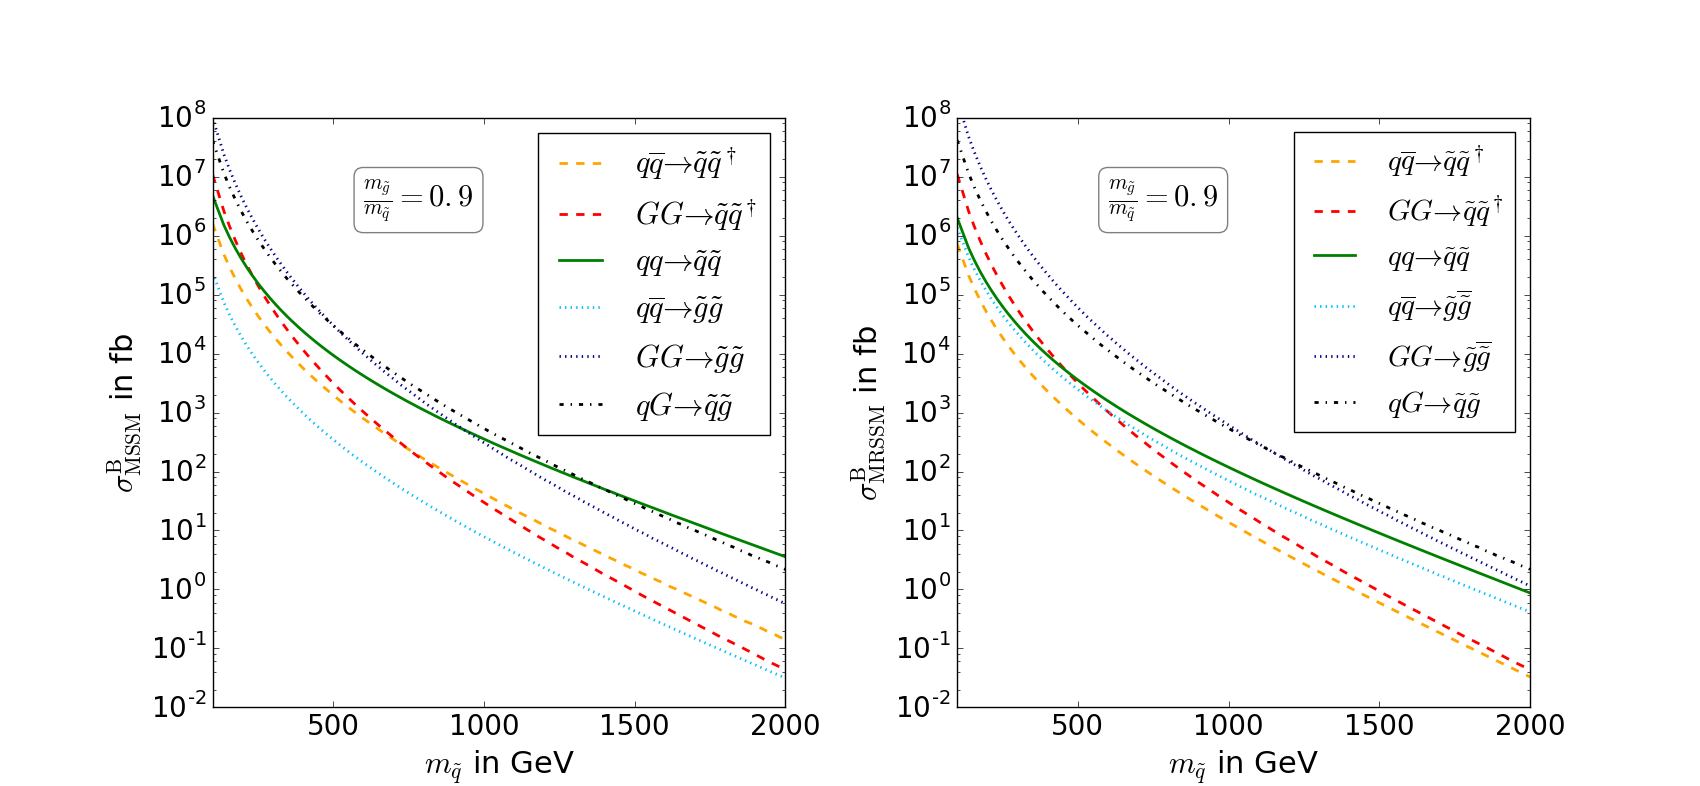
\includegraphics[scale=.4]{figures/mr=0,9_MSSM+MRSSM}
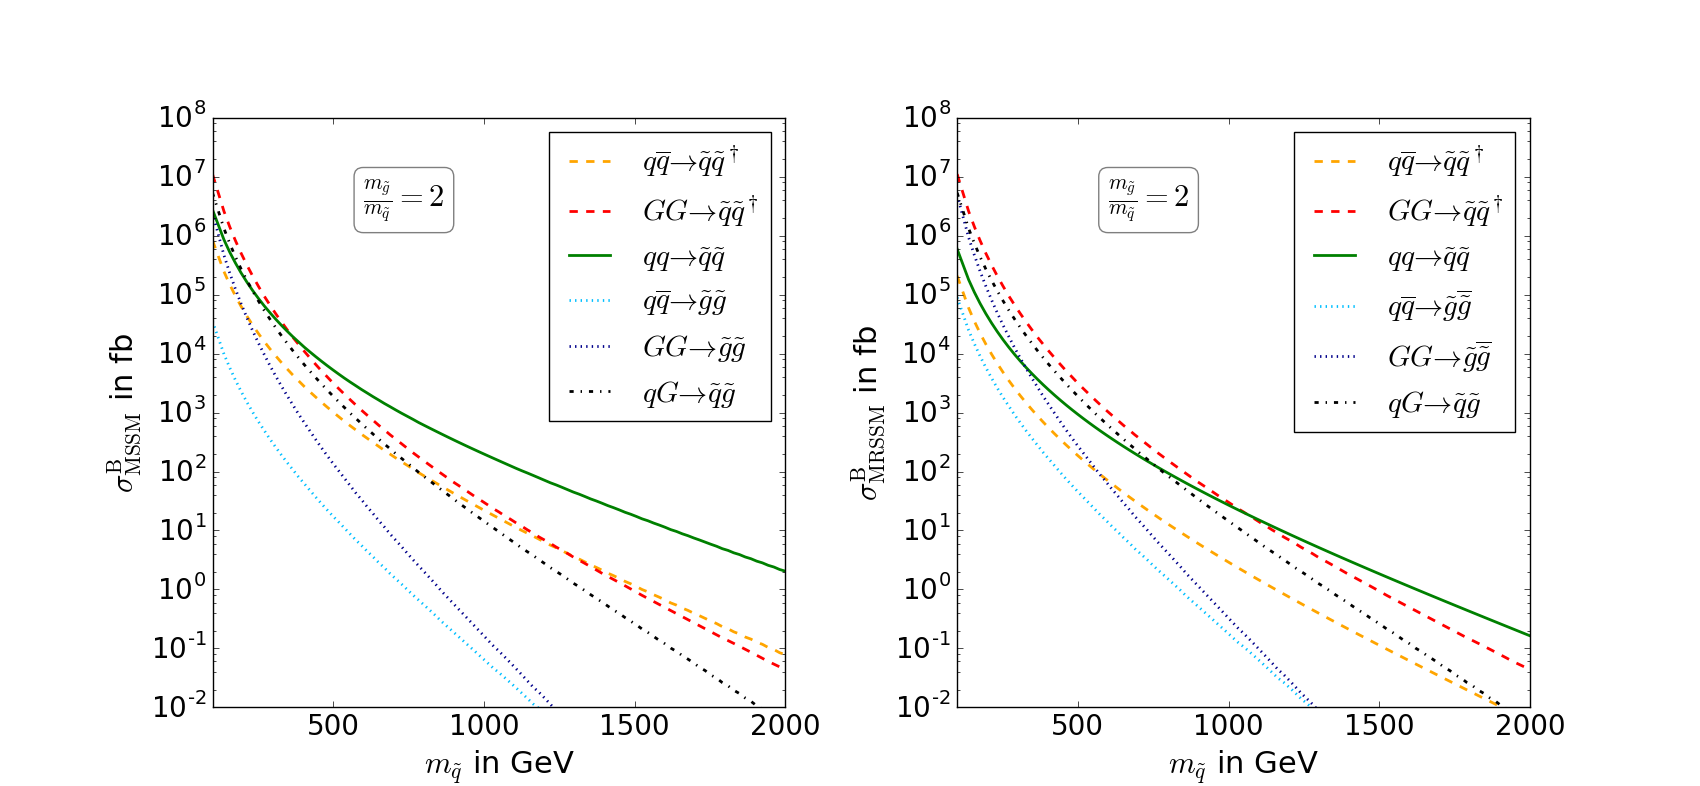
\includegraphics[scale=.4]{figures/mr=2_MSSM+MRSSM}
\caption{Hadronic cross section for squark and gluino production in the MSSM (left-hand side) and MRSSM (right-hand side) at the LHC at $\sqrt{S} = \unit[13]{GeV}$. The ratio of gluino and squark mass is fixed to 0.9 (first row) and 2 (second row). In the final state it has been summed over all squark flavors expect for staus. For the channels $qq \to \tilde{q}\tilde{q}$ and $qG \to \tilde{q}\tilde{G}$ also the charge conjugated process is included. The parton densities used are $\mathtt{MMHT2014}$ LO with $\alpha_s(M_Z) = 0.135$ in the 5-flavor scheme \cite{Harland-Lang:2014zoa}. As renormalization and factorization scale $\mu_R = \mu_F = \frac{m_1 + m_2}{2}$ has been chosen, where $m_i$ are the final state particle masses.} \label{fig:TreeXsection}
\end{center}
\end{figure}


\subsubsection*{The process $q_i \overline{q}_j \to \tilde{q}\tilde{q}^\dagger$}
The production of a squark and an antisquark through a quark and an antiquark in the initial state originates from two types of Feynman diagrams. The first one has an $s$-channel gluon and is the same in the MSSM and in the MRSSM. The second one exhibits a difference due to the $t$-channel gluino which is no Majorana particle in the MRSSM. 
\begin{figure}[!htbp]
\begin{center}
\begin{tikzpicture}[line width=1.0 pt, scale=1.3]
	\draw[fermion] (-1,0.5)--(-0.42,0);
	\draw[fermionbar] (-1,-0.5)--(-0.42,0);
	\draw[gluon] (-0.42,0)--(0.42,0); 
	\draw[scalar] (0.42,0)--(1,0.5);
	\draw[scalarbar] (0.42,0)--(1,-0.5);
\begin{scope}[shift={(3,0)}]
	\draw[fermion] (-1,0.5)--(0,0.5);
	\draw[fermionbar] (-1,-0.5)--(0,-0.5);
	\draw[fermionnoarrow] (0,0.5)--(0,-0.5);
	\draw[gluon] (0,0.5)--(0,-0.5); 
	\draw[scalar] (0,0.5)--(1,0.5);
	\draw[scalarbar] (0,-0.5)--(1,-0.5);
\end{scope}
\end{tikzpicture}
\caption{Tree level diagrams for $q\overline{q} \to \tilde{q}\tilde{q}^\dagger$}
\end{center}
\end{figure}
To see this one can either just apply the Feynman rules in Appendix \ref{sec:FeynmanRules} or think of the conservation of R-charge: Left handed squarks have R-charge +1 and right handed squarks have R-charge -1. Antiparticles have the opposite R-charge of their corresponding particles. The final state particles have to meet the total R-charge zero from the initial state. Because of this one only has $\tilde{q}_L \overline{\tilde{q}}_L$ and $\tilde{q}_R \overline{\tilde{q}}_R$ as the final states in the MRSSM whereas in the MSSM one actually has four instead of two t-channel diagrams: The corresponding final states are $\tilde{q}_L \overline{\tilde{q}}_L$, $\tilde{q}_R \overline{\tilde{q}}_R$, $\tilde{q}_L \overline{\tilde{q}}_R$ and $\overline{\tilde{q}}_R \tilde{q}_L$. Consequently contributions from the $t$-channel diagrams are suppressed in the MRSSM in comparison to the MSSM. As visible in fig. \ref{fig:TreeXsection} this suppression grows with the masses. The reason for this lies in the gluino mass dependence of the $t$-channel diagrams which is explained in the discussion of squark production.\\
If the initial state quarks are of different flavor the $s$-channel diagram is absent.

\subsubsection*{The process $GG \to \tilde{q}\tilde{q}^\dagger$}
This process has the same cross section in the MRSSM and in the MSSM for also in the MSSM only like chirality squark and antisquark $\tilde{q}_A\tilde{q}_A^\dagger$ with $A \in {L,R}$ can be produced

\subsubsection*{The process $q_i q_j \to \tilde{q}\tilde{q}$}
In the MRSSM only the production of unlike chirality squarks $\tilde{q}_L \tilde{q}_R$ is allowed whilst in the MSSM also like chirality squarks can be produced. This is again a consequence of the conservation of R-charge. The upshot of this is a suppression of squark production in the MRSSM in comparison to the MSSM. To be more explicit the suppression of squark production in the MRSSM grows with the gluino mass. This can be understood as follows: As in the MRSSM a left handed squark needs to be produced with a right handed squark one can read off from the Feynman rules given in Appendix \ref{sec:FeynmanRules} that the gluino propagator $i\frac{\slashed{p}+m_{\tilde{g}}}{p^2-m_{\tilde{g}}^2}$ is sandwiched between the projectors $P_L$ and $P_R$ which leads to the cancellation of the gluino mass in the numerator. Therefore for small momenta of the gluino compared to the gluino mass one gets $\mathcal{M}$ $\sim \frac{1}{m_{\tilde{g}}^2}$ in the MRSSM while in the MSSM one finds a suppression proportional to $\frac{1}{m_{\tilde{g}}}$.\\
When considering squark production one has to sum over all $|\mathcal{M}|^2$ with different helicity. The diagrams for those different final state helicities are shown for flavor like squark production in tab. \ref{tab:squark_likeflavor} and for flavor unlike squark production in tab. \ref{tab:squark_unlikeflavor} for the MSSM and the MRSSM. To avoid double counting one needs to weight $|\mathcal{M}|^2(qq\to \tilde{q}_L\tilde{q}_L)$ and $|\mathcal{M}|^2(qq\to \tilde{q}_R\tilde{q}_R)$ with a statistical factor of $\frac{1}{2}$ as one integrates over all momenta of both particles to arrive at the cross section.\footnote{Alternatively one could discard the $u$-channel (or $t$-channel) diagram and omit the weighting with $\frac{1}{2}$.}
\begin{table}[!htpb]
\begin{center}
\begin{tabular}{c|c}
MSSM & MRSSM \\
\hline
\begin{tikzpicture}[line width=1.0 pt, scale=0.7]
	\draw[fermion] (0,1)--(1,1);
	\draw[fermion] (0,0)--(1,0);
	\draw[fermionnoarrow] (1,1)--(1,0);
	\draw[gluon] (1,1)--(1,0);
	\draw[scalar] (1,1)--(2,1);
	\draw[scalar] (1,0)--(2,0);
	\node at (-0.2,1) {$u$};
	\node at (-0.2,0) {$u$};
	\node at (2.2,1) {$\tilde{u}_L^\dagger$};
	\node at (2.2,0) {$\tilde{u}_R^\dagger$};
\begin{scope}[shift={(4,0)}]
	\draw[fermion] (0,1)--(1,1);
	\draw[fermion] (0,0)--(1,0);
	\draw[fermionnoarrow] (1,1)--(1,0);
	\draw[gluon] (1,1)--(1,0);
	\draw[scalar] (1,1)--(1.5,0.5);
	\draw[scalar] (1.5,0.5)--(2,0);
	\draw[scalar] (1,0)--(1.4,0.4);
	\draw[scalar] (1.6,0.6)--(2,1);
	\node at (-0.2,1) {$u$};
	\node at (-0.2,0) {$u$};
	\node at (2.2,1) {$\tilde{u}_L^\dagger$};
	\node at (2.2,0) {$\tilde{u}_R^\dagger$};
\end{scope}
\begin{scope}[shift={(0,-2)}]
	\draw[fermion] (0,1)--(1,1);
	\draw[fermion] (0,0)--(1,0);
	\draw[fermionnoarrow] (1,1)--(1,0);
	\draw[gluon] (1,1)--(1,0);
	\draw[scalar] (1,1)--(2,1);
	\draw[scalar] (1,0)--(2,0);
	\node at (-0.2,1) {$u$};
	\node at (-0.2,0) {$u$};
	\node at (2.2,1) {$\tilde{u}_L^\dagger$};
	\node at (2.2,0) {$\tilde{u}_L^\dagger$};
\end{scope}
\begin{scope}[shift={(4,-2)}]
	\draw[fermion] (0,1)--(1,1);
	\draw[fermion] (0,0)--(1,0);
	\draw[fermionnoarrow] (1,1)--(1,0);
	\draw[gluon] (1,1)--(1,0);
	\draw[scalar] (1,1)--(1.5,0.5);
	\draw[scalar] (1.5,0.5)--(2,0);
	\draw[scalar] (1,0)--(1.4,0.4);
	\draw[scalar] (1.6,0.6)--(2,1);
	\node at (-0.2,1) {$u$};
	\node at (-0.2,0) {$u$};
	\node at (2.2,1) {$\tilde{u}_L^\dagger$};
	\node at (2.2,0) {$\tilde{u}_L^\dagger$};
\end{scope}
\begin{scope}[shift={(0,-4)}]
	\draw[fermion] (0,1)--(1,1);
	\draw[fermion] (0,0)--(1,0);
	\draw[fermionnoarrow] (1,1)--(1,0);
	\draw[gluon] (1,1)--(1,0);
	\draw[scalar] (1,1)--(2,1);
	\draw[scalar] (1,0)--(2,0);
	\node at (-0.2,1) {$u$};
	\node at (-0.2,0) {$u$};
	\node at (2.2,1) {$\tilde{u}_R^\dagger$};
	\node at (2.2,0) {$\tilde{u}_R^\dagger$};
\end{scope}
\begin{scope}[shift={(4,-4)}]
	\draw[fermion] (0,1)--(1,1);
	\draw[fermion] (0,0)--(1,0);
	\draw[fermionnoarrow] (1,1)--(1,0);
	\draw[gluon] (1,1)--(1,0);
	\draw[scalar] (1,1)--(1.5,0.5);
	\draw[scalar] (1.5,0.5)--(2,0);
	\draw[scalar] (1,0)--(1.4,0.4);
	\draw[scalar] (1.6,0.6)--(2,1);
	\node at (-0.2,1) {$u$};
	\node at (-0.2,0) {$u$};
	\node at (2.2,1) {$\tilde{u}_R^\dagger$};
	\node at (2.2,0) {$\tilde{u}_R^\dagger$};
\end{scope}
\end{tikzpicture} & \begin{tikzpicture}[line width=1.0 pt, scale=0.7]
	\draw[fermion] (0,1)--(1,1);
	\draw[fermion] (0,0)--(1,0);
	\draw[fermionnoarrow] (1,1)--(1,0);
	\draw[gluon] (1,1)--(1,0);
	\draw[scalar] (1,1)--(2,1);
	\draw[scalar] (1,0)--(2,0);
	\node at (-0.2,1) {$u$};
	\node at (-0.2,0) {$u$};
	\node at (2.2,1) {$\tilde{u}_L^\dagger$};
	\node at (2.2,0) {$\tilde{u}_R^\dagger$};
\begin{scope}[shift={(4,0)}]
	\draw[fermion] (0,1)--(1,1);
	\draw[fermion] (0,0)--(1,0);
	\draw[fermionnoarrow] (1,1)--(1,0);
	\draw[gluon] (1,1)--(1,0);
	\draw[scalar] (1,1)--(1.5,0.5);
	\draw[scalar] (1.5,0.5)--(2,0);
	\draw[scalar] (1,0)--(1.4,0.4);
	\draw[scalar] (1.6,0.6)--(2,1);
	\node at (-0.2,1) {$u$};
	\node at (-0.2,0) {$u$};
	\node at (2.2,1) {$\tilde{u}_L^\dagger$};
	\node at (2.2,0) {$\tilde{u}_R^\dagger$};
\end{scope}
\begin{scope}[shift={(0,-4.3)}]
\node at (0,0) {};
\end{scope}
\end{tikzpicture} 
\end{tabular}
\caption{All Feynman diagrams contributing to flavor like squark production in the MSSM and the MRSSM for the example of $u$-quarks. For the MSSM the absolute squared Feynman amplitudes from the diagrams with chirality like squarks need to be weighted with a factor of $\frac{1}{2}$.}\label{tab:squark_likeflavor}
\end{center}
\end{table}
\begin{table}[!htpb]
\begin{center}
\begin{tabular}{c|c}
MSSM & MRSSM \\
\hline
\begin{tikzpicture}[line width=1.0 pt, scale=0.7]
	\draw[fermion] (0,1)--(1,1);
	\draw[fermion] (0,0)--(1,0);
	\draw[fermionnoarrow] (1,1)--(1,0);
	\draw[gluon] (1,1)--(1,0);
	\draw[scalar] (1,1)--(2,1);
	\draw[scalar] (1,0)--(2,0);
	\node at (-0.2,1) {$u$};
	\node at (-0.2,0) {$d$};
	\node at (2.2,1) {$\tilde{u}_L^\dagger$};
	\node at (2.2,0) {$\tilde{d}_R^\dagger$};
\begin{scope}[shift={(4,0)}]
	\draw[fermion] (0,1)--(1,1);
	\draw[fermion] (0,0)--(1,0);
	\draw[fermionnoarrow] (1,1)--(1,0);
	\draw[gluon] (1,1)--(1,0);
	\draw[scalar] (1,1)--(2,1);
	\draw[scalar] (1,0)--(2,0);
	\node at (-0.2,1) {$u$};
	\node at (-0.2,0) {$d$};
	\node at (2.2,1) {$\tilde{u}_R^\dagger$};
	\node at (2.2,0) {$\tilde{d}_L^\dagger$};
\end{scope}
\begin{scope}[shift={(0,-2)}]
	\draw[fermion] (0,1)--(1,1);
	\draw[fermion] (0,0)--(1,0);
	\draw[fermionnoarrow] (1,1)--(1,0);
	\draw[gluon] (1,1)--(1,0);
	\draw[scalar] (1,1)--(2,1);
	\draw[scalar] (1,0)--(2,0);
	\node at (-0.2,1) {$u$};
	\node at (-0.2,0) {$d$};
	\node at (2.2,1) {$\tilde{u}_L^\dagger$};
	\node at (2.2,0) {$\tilde{d}_L^\dagger$};
\end{scope}
\begin{scope}[shift={(0,-4)}]
	\draw[fermion] (0,1)--(1,1);
	\draw[fermion] (0,0)--(1,0);
	\draw[fermionnoarrow] (1,1)--(1,0);
	\draw[gluon] (1,1)--(1,0);
	\draw[scalar] (1,1)--(2,1);
	\draw[scalar] (1,0)--(2,0);
	\node at (-0.2,1) {$u$};
	\node at (-0.2,0) {$d$};
	\node at (2.2,1) {$\tilde{u}_R^\dagger$};
	\node at (2.2,0) {$\tilde{d}_R^\dagger$};
\end{scope}
\end{tikzpicture} & \begin{tikzpicture}[line width=1.0 pt, scale=0.7]
	\draw[fermion] (0,1)--(1,1);
	\draw[fermion] (0,0)--(1,0);
	\draw[fermionnoarrow] (1,1)--(1,0);
	\draw[gluon] (1,1)--(1,0);
	\draw[scalar] (1,1)--(2,1);
	\draw[scalar] (1,0)--(2,0);
	\node at (-0.2,1) {$u$};
	\node at (-0.2,0) {$d$};
	\node at (2.2,1) {$\tilde{u}_L^\dagger$};
	\node at (2.2,0) {$\tilde{d}_R^\dagger$};
\begin{scope}[shift={(4,0)}]
	\draw[fermion] (0,1)--(1,1);
	\draw[fermion] (0,0)--(1,0);
	\draw[fermionnoarrow] (1,1)--(1,0);
	\draw[gluon] (1,1)--(1,0);
	\draw[scalar] (1,1)--(2,1);
	\draw[scalar] (1,0)--(2,0);
	\node at (-0.2,1) {$u$};
	\node at (-0.2,0) {$d$};
	\node at (2.2,1) {$\tilde{u}_R^\dagger$};
	\node at (2.2,0) {$\tilde{d}_L^\dagger$};
\end{scope}
\begin{scope}[shift={(0,-4.3)}]
\node at (0,0) {};
\end{scope}
\end{tikzpicture} 
\end{tabular}
\caption{All Feynman diagrams contributing to flavor unlike squark production in the MSSM and the MRSSM for the example of $u$- and $d$-quarks.}\label{tab:squark_unlikeflavor}
\end{center}
\end{table}\\
Because of the absence of chirality like squarks in the final state in the MRSSM (and a missing interference of the two diagrams in tab. \ref{tab:squark_likeflavor} in the MRSSM) the cross section of flavor like and unlike squarks is the same in the MRSSM, i.e. on the partonic level:\\ $\sigma^{\mathrm{B}}_{\mathrm{Part,\ MRSSM}}(\tilde{u}_L\tilde{u}_R) = \sigma^{\mathrm{B}}_{\mathrm{Part,\ MRSSM}}(\tilde{u}_L\tilde{d}_R)$. That is however not true in the MSSM. 


\subsubsection*{The process $q \overline{q} \to \tilde{g}\overline{\tilde{g}}$}
In contrast to the MSSM no statistical factor of $\frac{1}{2}$ is taken into account when turning from $|\mathcal{M}|^2$ to $\sigma$. This is because gluino and antigluino are distinguishable particles. Still in comparison to the MSSM cross section only the first line in \ref{eq:qqbar_to_sgsgbar} is doubled up as the other two lines origin from an $t$ or $u$ channel squark which occurs in only one instead of two chiralities. Furthermore an interference term from the $t$ or $u$ channel diagram which occurs in the MSSM is absent in the MRSSM.
% this interference term causes a huge difference, that's been checked by Philip via Madgraph

\subsubsection*{The process $GG \to \tilde{g}\overline{\tilde{g}}$}
As in the previous process the MRSSM cross section for $GG \to \tilde{g}\overline{\tilde{g}}$ receives no statistical factor of $\frac{1}{2}$. As there are no further differences between MSSM and MRSSM in this channel, the MRSSM cross section is simply twice as large as in the MSSM.

\subsubsection*{The process $q G \to \tilde{q} \tilde{g}$}
This process is exactly the same in the MSSM and MRSSM.
\\
refer to Vernoica Sanz: How many SUpersymmetries?

\begin{figure}[!htpb]
\begin{center}
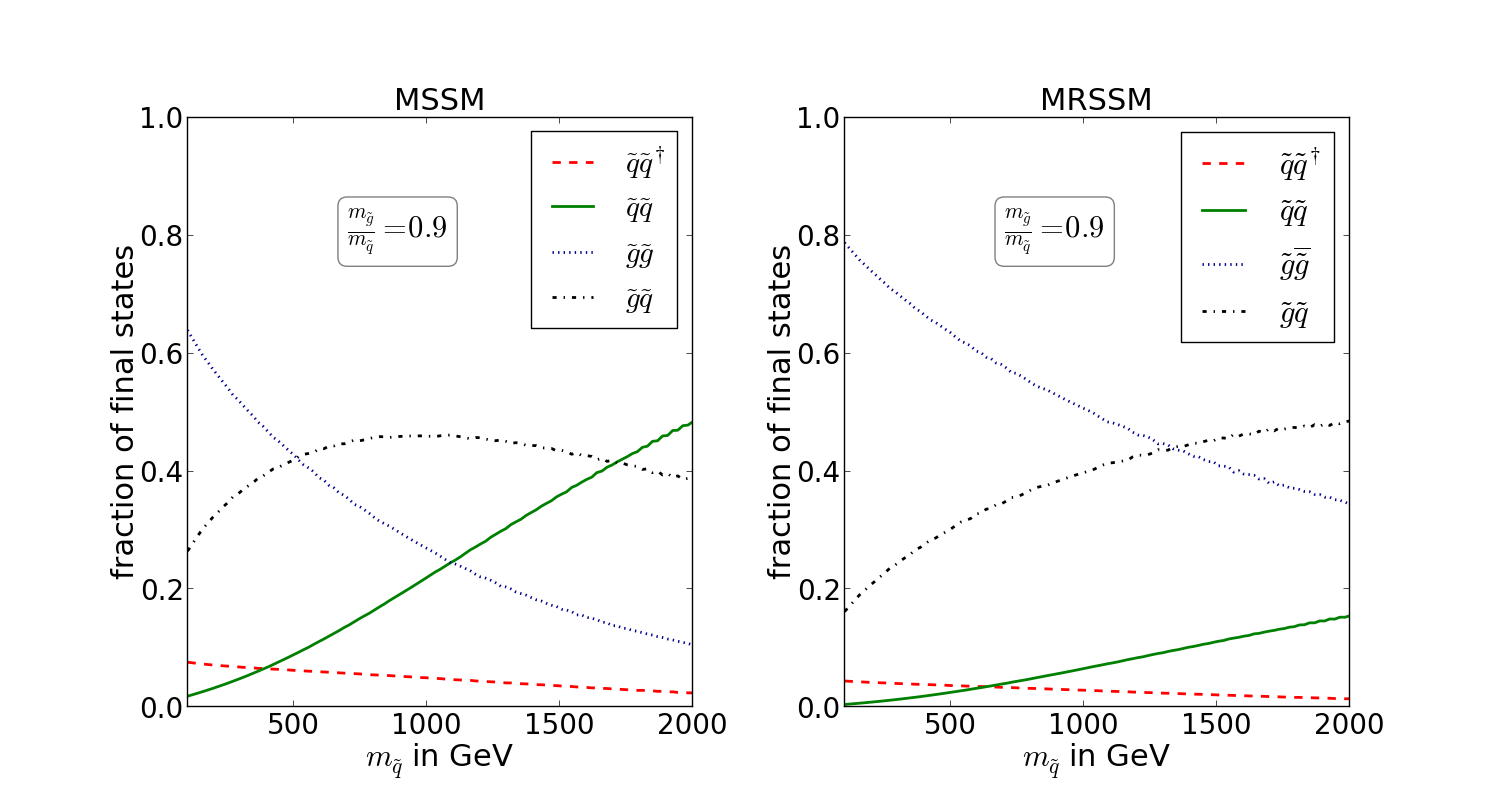
\includegraphics[scale=.45]{figures/rel_weights_mr=0,9_MSSM+MRSSM}
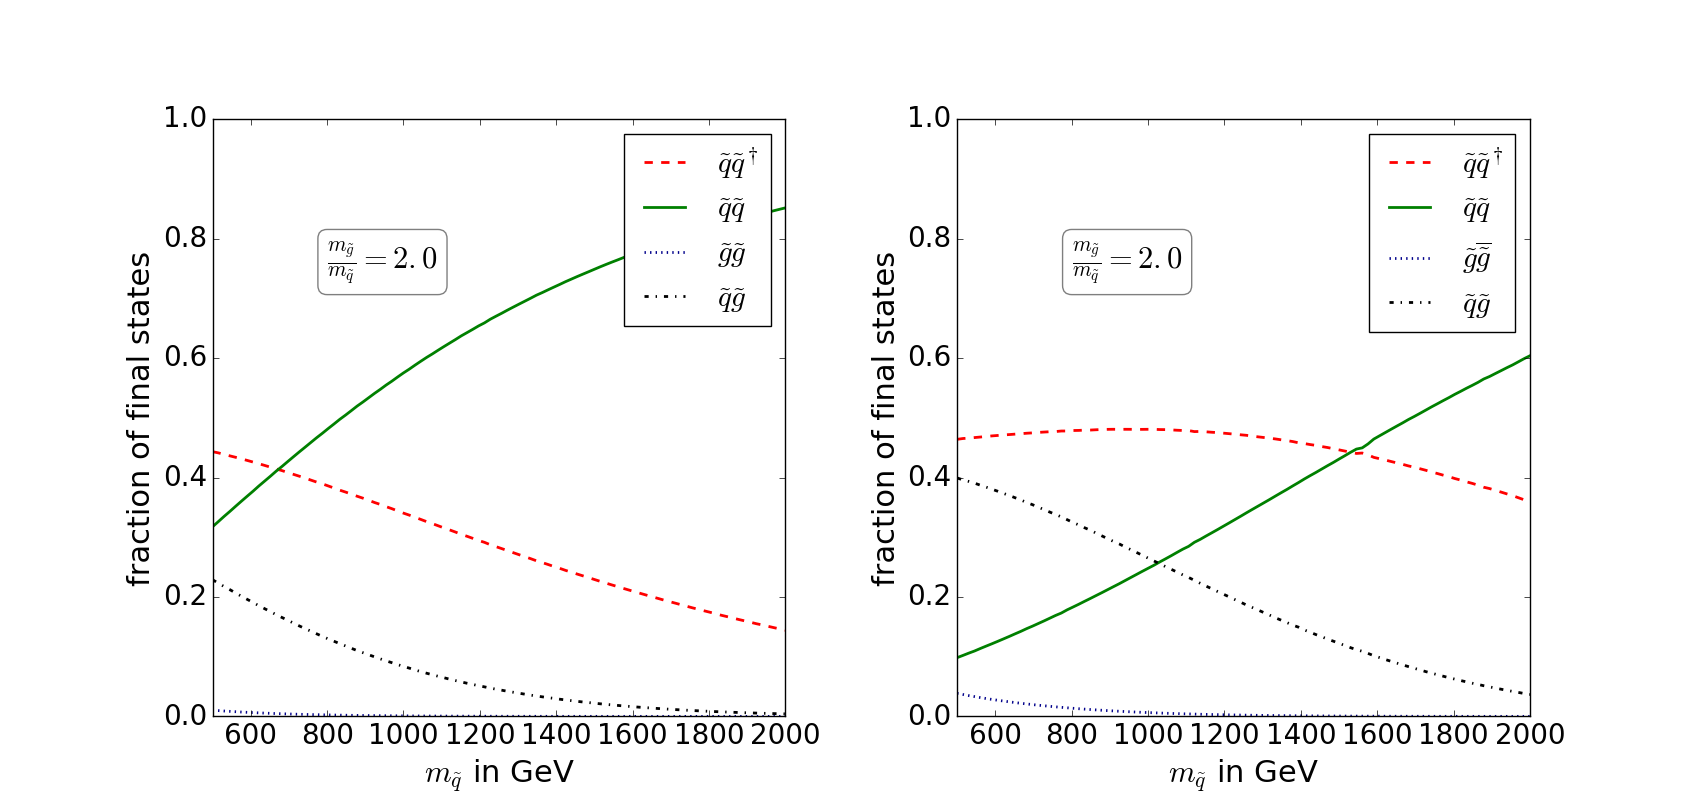
\includegraphics[scale=.45]{figures/rel_weights_mr=2_MSSM+MRSSM}
\caption{Relative contributions of the indicated final states on the total hadronic cross section in the MSSM (left-hand side) and MRSSM (right-hand side) at the LHC at $\sqrt{S} = \unit[13]{GeV}$. The ratio of gluino and squark mass is fixed to 0.9 (first row) and 2 (second row). In the final state it has been summed over all squark flavors expect for staus. For the channels $qq \to \tilde{q}\tilde{q}$ and $qG \to \tilde{q}\tilde{G}$ also the charge conjugated process is included. The parton densities and the renormalization and factorization scale are chosen as in fig. \ref{fig:TreeXsection}.}\label{fig:TreeLevelSigma_0,9_2}
\end{center}
\end{figure}

\begin{figure}[!htpb]
\begin{center}
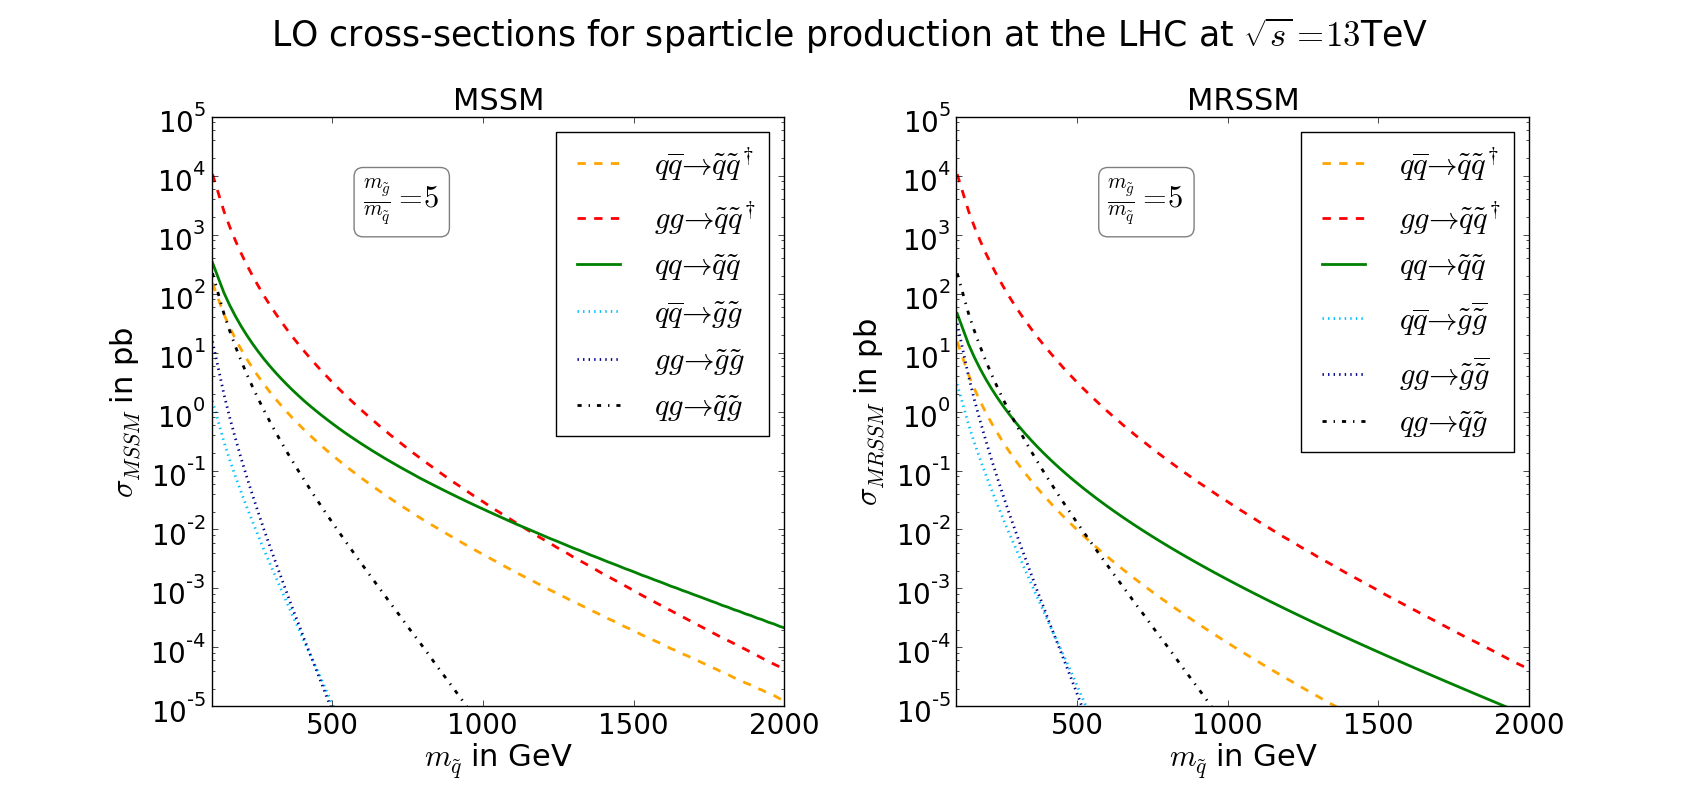
\includegraphics[scale=.4]{figures/mr=5_MSSM+MRSSM}
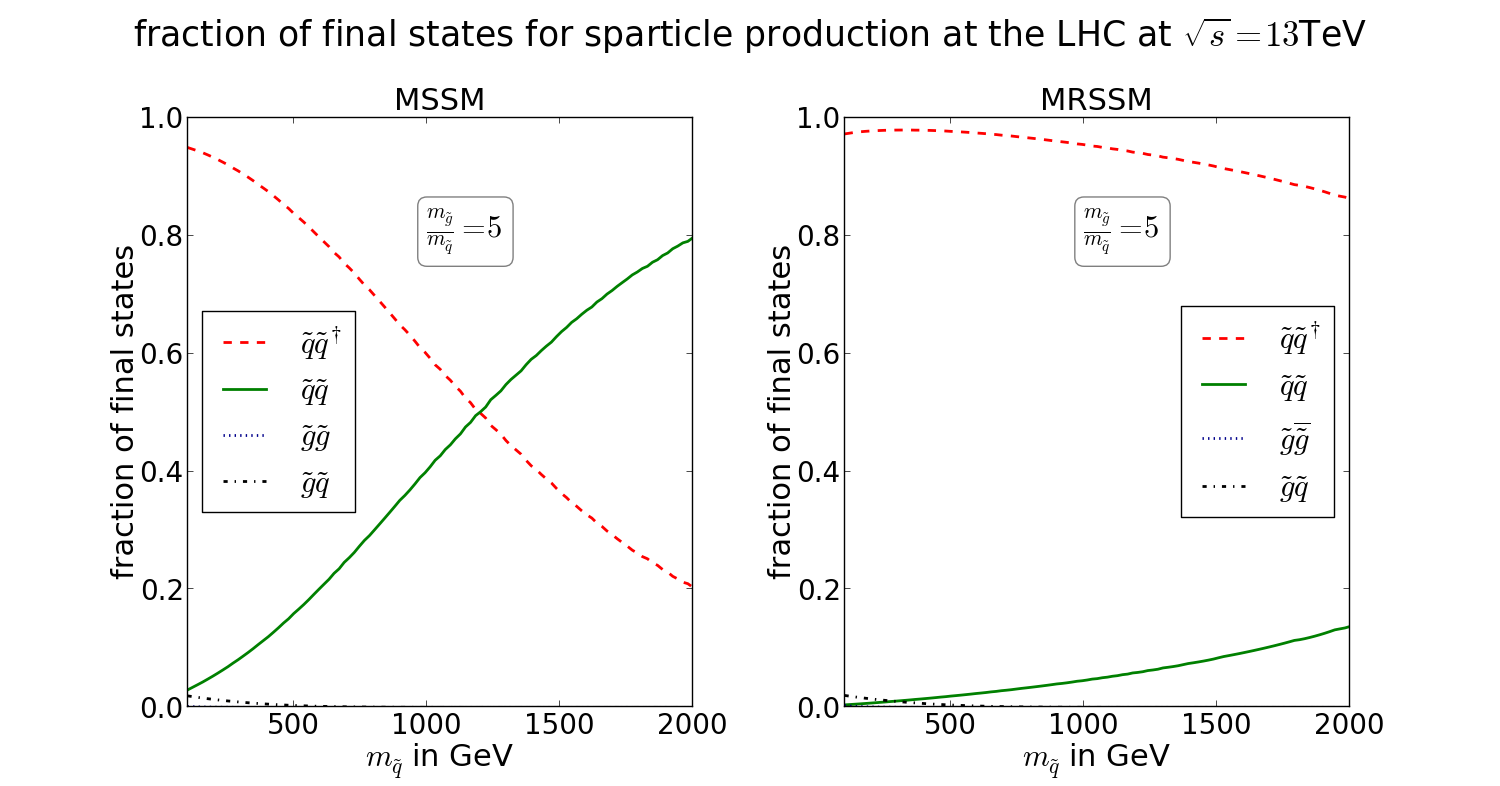
\includegraphics[scale=.45]{figures/rel_weights_mr=5_MSSM+MRSSM}
\caption{Hadronic cross section for squark and gluino production (in the first row) and relative contributions of the indicated final states on the total hadronic cross section in the MSSM (left-hand side) and MRSSM (right-hand side) at the LHC at $\sqrt{S} = \unit[13]{GeV}$. The ratio of gluino and squark mass is fixed to 5. In the final state it has been summed over all squark flavors expect for staus. For the channels $qq \to \tilde{q}\tilde{q}$ and $qG \to \tilde{q}\tilde{G}$ also the charge conjugated process is included. The parton densities and the renormalization and factorization scale are chosen as in fig. \ref{fig:TreeXsection}.}
\end{center}
\end{figure}


\begin{figure}[!htpb]
\begin{center}
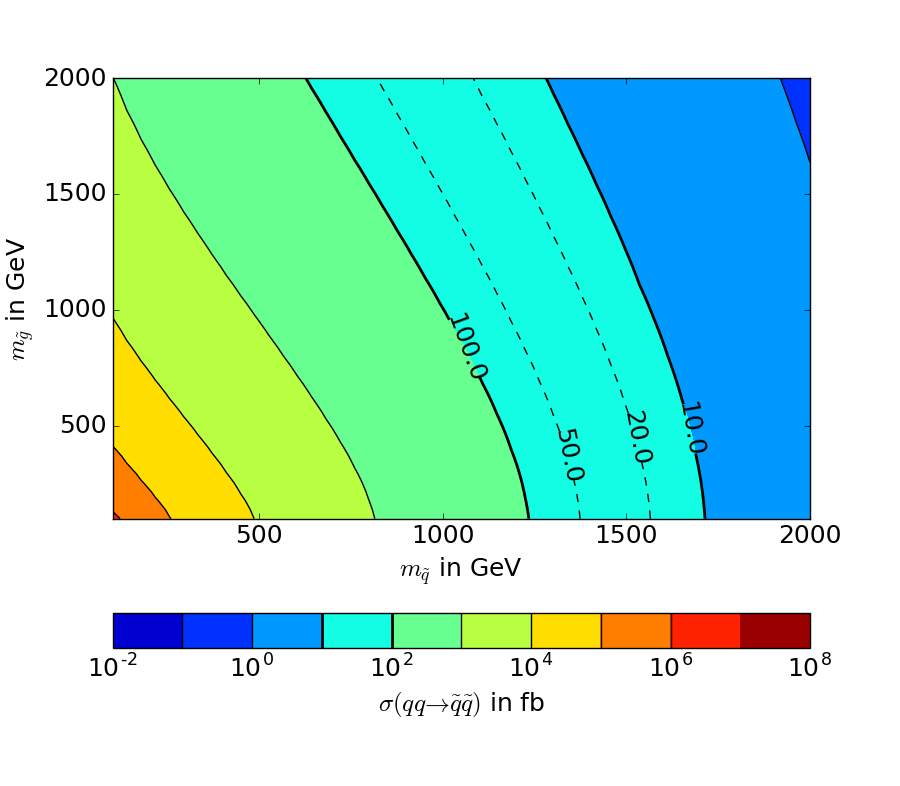
\includegraphics[scale=.6]{figures/contour_MRSSM_squarks}
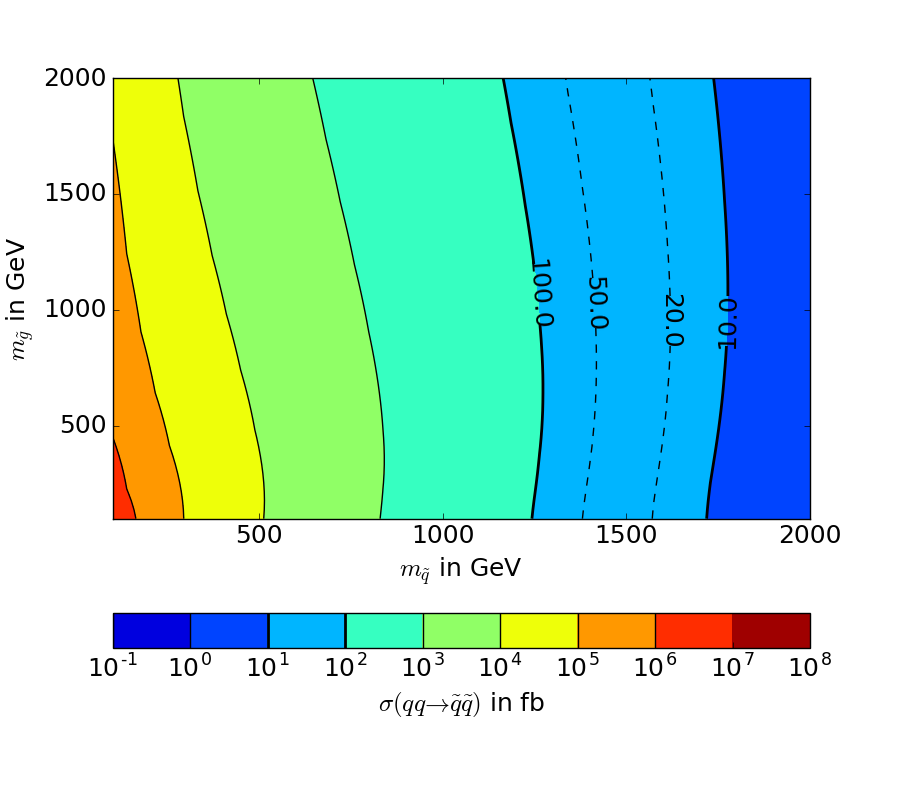
\includegraphics[scale=.6]{figures/contour_MSSM_squarks}
\caption{}
\end{center}
\end{figure}

\begin{figure}[!htpb]
\begin{center}
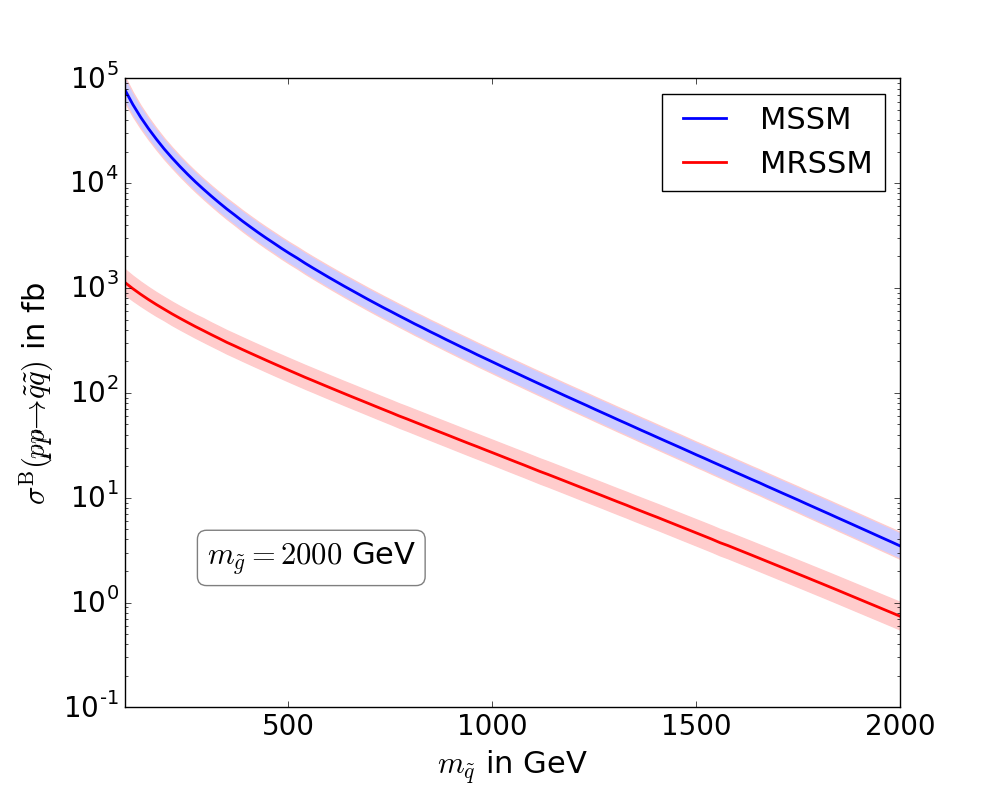
\includegraphics[scale=.5]{figures/MSSM+MRSSM_msg=2000}
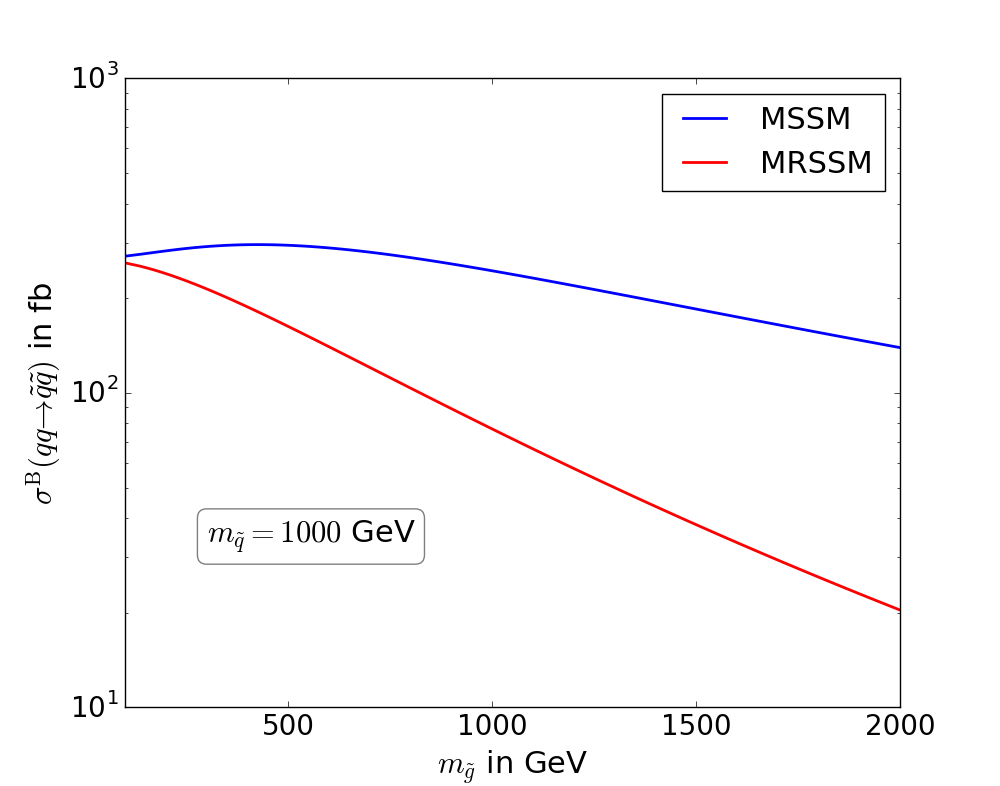
\includegraphics[scale=.5]{figures/MSSM+MRSSM_msq=1000}
\caption{add error bars}
\end{center}
\end{figure}
